\documentclass{article}

\usepackage{graphicx}
\usepackage{tikz}
\usepackage{tikzsymbols}
\usetikzlibrary{calc,patterns,shapes.geometric}
\pagestyle{empty}
\usepackage[margin=0pt]{geometry}
\geometry{papersize={14in,12in}}

\def\centerarc[#1](#2)(#3:#4:#5){\draw[#1] ($(#2)+({#5*cos(#3)},{#5*sin(#3)})$) arc (#3:#4:#5);}

\begin{document}
	\begin{figure}
		\centering
		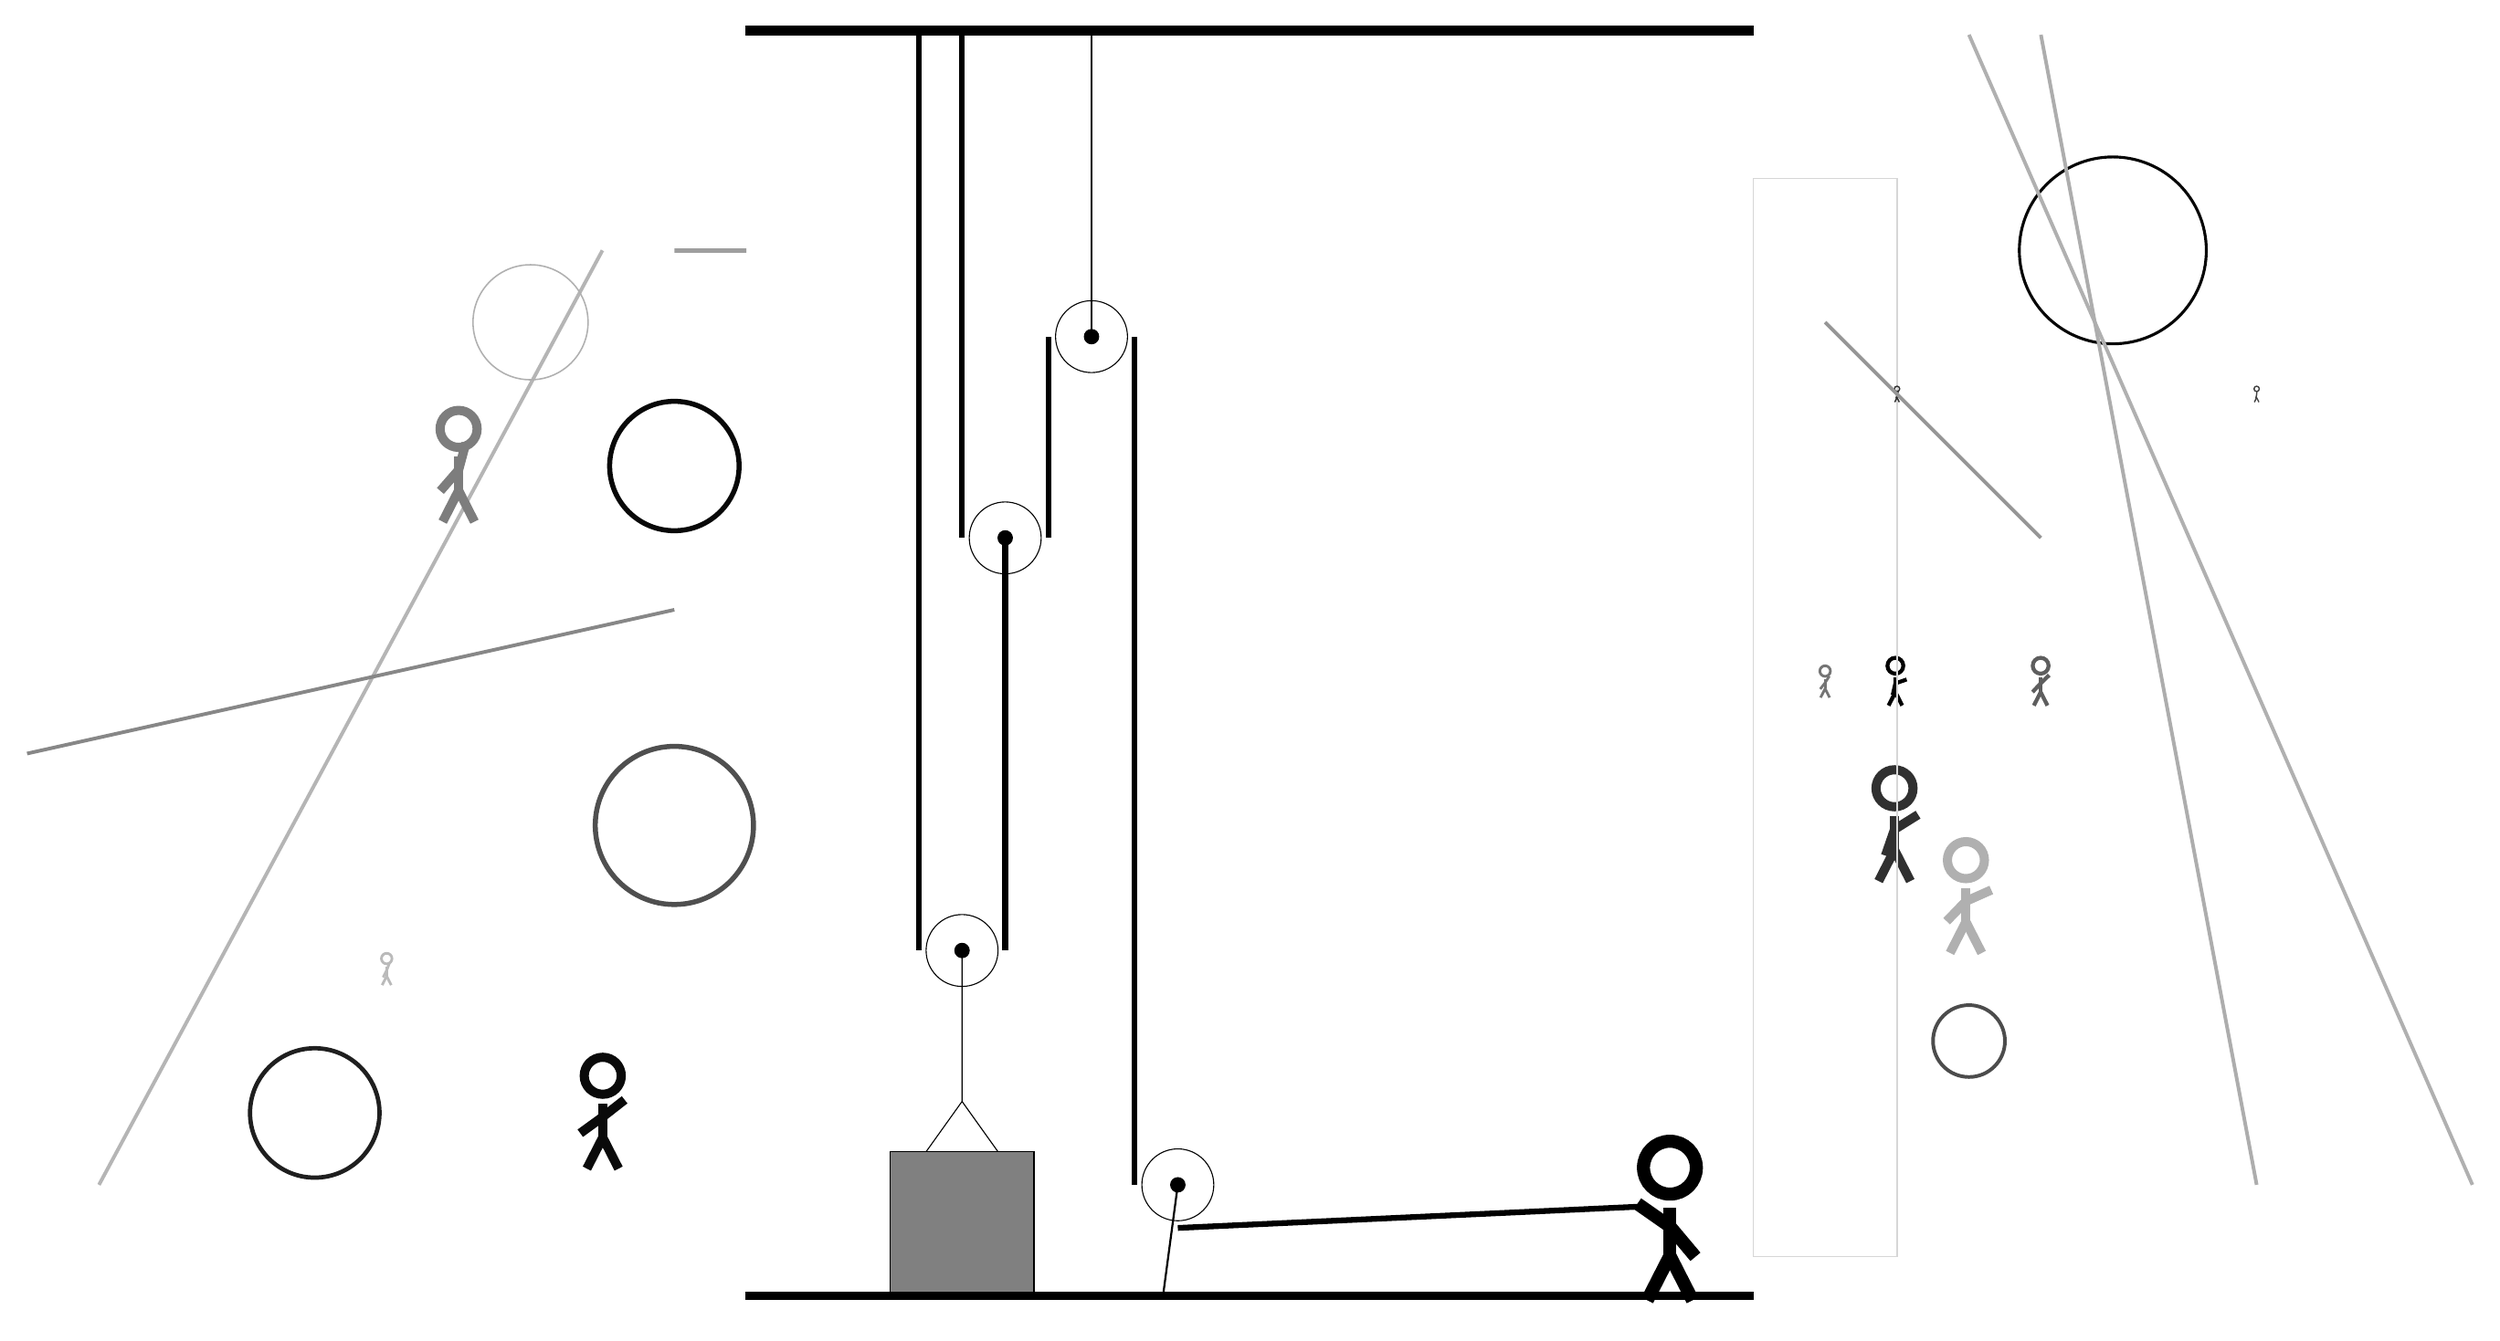
\begin{tikzpicture}
			%%%%% START %%%%%
			
			\draw[fill=black] (-2, 14) rectangle (12, 14.125);
			
			\draw (1, 1.26) circle (0.5);
			\draw[fill=black] (1, 1.26) circle (0.1);
			
			\draw (1.6, 7.0) circle (0.5);
			\draw[fill=black] (1.6, 7.0) circle (0.1);
			
			\draw [line width=0.5mm, color=black!70](15, 0) circle (0.5);
			
			\node[line width=0.3mm, color=black!27] at (-7, 1) {\Strichmaxerl[2][63][69]};
			\draw[line width=0.5mm, color=black!29](-4, 11) -- (-11, -2);
			\node[line width=0.3mm, color=black!51] at (-6, 8) {\Strichmaxerl[7][49][75]};
			\draw [line width=0.4mm, color=black!98](17, 11) circle (1.3);
			\node[line width=0.6mm, color=black!74] at (19, 9) {\Strichmaxerl[1][77][86]};
			
			\draw[line width=0.5mm, color=black!31](15, 14) -- (22, -2);
			
			\node[line width=0.7mm, color=black!81] at (14, 3) {\Strichmaxerl[7][71][32]};
			\node[line width=0.4mm, color=black!100] at (14, 5) {\Strichmaxerl[3][77][19]};
			\draw[line width=0.5mm, color=black!32](16, 14) -- (19, -2);
			\draw[line width=0.7mm, color=black!38] (-3, 11) rectangle (-2, 11);
			
			\draw [line width=0.7mm, color=black!97](-3, 8) circle (0.9);
			\node[line width=0.4mm, color=black!96] at (-4, -1) {\Strichmaxerl[7][36][38]};
			
			\draw[line width=0.2mm, color=black!16] (12, -3) rectangle (14, 12);
			\draw [line width=0.7mm, color=black!69](-3, 3) circle (1.1);
			\node[line width=0.3mm, color=black!54] at (13, 5) {\Strichmaxerl[2][52][58]};
			
			\draw[line width=0.5mm, color=black!47](-3, 6) -- (-12, 4);
			
			\draw [line width=0.2mm, color=black!31](-5, 10) circle (0.8);
			\node[line width=0.3mm, color=black!81] at (14, 9) {\Strichmaxerl[1][74][69]};
			
			\node[line width=0.7mm, color=black!31] at (15, 2) {\Strichmaxerl[7][46][24]};
			\draw [line width=0.6mm, color=black!88](-8, -1) circle (0.9);
			
			\draw[line width=0.5mm, color=black!41](16, 7) -- (13, 10);
			
			\node[line width=0.2mm, color=black!63] at (16, 5) {\Strichmaxerl[3][47][44]};
			
			\draw (2.8, 9.8) circle (0.5);
			\draw[fill=black] (2.8, 9.8) circle (0.1);
			\draw[thick] (2.8, 9.8) -- (2.8, 14);
			
			\draw (4.0, -2) circle (0.5);
			\draw[fill=black] (4.0, -2) circle (0.1);
			\draw[thick] (4.0, -2) -- (3.8, -3.5);
			
			\draw (1, 1.26) -- (1, -0.84) -- (0.5, -1.54) -- (1.5, -1.54) -- (1, -0.84);
			\draw[fill=black!50] (0, -1.54) rectangle (2, -3.54);
			\draw[line width=0.8mm] (0.4, 14) -- (0.4, 1.26);
			\centerarc[line width=0.8mm](1, 1.26)(180:360:0.6);
			\draw[line width=0.8mm](1.6, 1.26) -- (1.6, 7.0);
			\draw[line width=0.8mm] (1.0, 14) -- (1.0, 7.0);
			\centerarc[line width=0.8mm](1.6, 7.0)(180:360:0.6);
			\draw[line width=0.8mm](2.2, 7.0) -- (2.2, 9.8);
			\centerarc[line width=0.8mm](2.8, 9.8)(0:180:0.6);
			\draw[line width=0.8mm] (3.4, 9.8) -- (3.4, -2);
			\centerarc[line width=0.8mm](4.0, -2)(0:90:-0.6);
			\draw[line width=0.8mm](4.0, -2.6) -- (10.5, -2.3);
			
			\node at (10.8, -2.5) {\Strichmaxerl[10][-35][-50]};
			
			\draw[fill=black] (-2, -3.5) rectangle (12, -3.6);
			
			%%%%% END %%%%%
		\end{tikzpicture}
	\end{figure}	
\end{document}